\section{Information flows in the DGA}
\label{sec:dga_flows}

In this Section, a detailed description of the DGA and its core legislative objectives is provided, including the introduction of use cases where Semantic Web technologies and decentralised data environments can be leveraged to aid data intermediaries and data altruism organisations to implement their services while fulfilling their renewed legal duties, in particular, related to the reporting of their activities and how they use personal and non-personal data from data subjects and data holders, respectively.

In February 2020, the \cite{european_commission_communication_2020} introduced a series of regulatory proposals aimed at legislating the European strategy for data, encompassing a set of new regulatory proposals aimed at governing the utilisation of non-personal and public data, regulating digital services and markets, and fostering the creation of common European data spaces.
By prioritising data and ensuring its accessibility across sectors, this transformation must also maintain the interests of both data subjects and data holders, while supporting trusted entities to facilitate data sharing aligned with new regulations.
Among these proposals was the Data Governance Act \citeyearpar{noauthor_regulation_2022}, a regulation presented to enhance data accessibility and foster trust in data intermediation services throughout the EU.
Following approval by both the European Parliament and the European Council, this legislation entered into force on 23 June 2022 and, following a 15 month grace period, has been applicable since September 2023.
Similarly to other data-related legislation within the EU, the DGA relays new rights and obligations to entities holding both personal and non-personal data.
It also regulates the operations of data users and two categories of data-related services related to data intermediation and altruism.
The principal objectives of this legislation include:

\begin{enumerate}
    \item[(i)] Facilitating the reuse of protected public-sector data while maintaining its privacy and confidentiality, particularly in cases where such data is subject to the rights of others, including trade secrets, personal data protection, and data safeguarded by intellectual property rights.
    \item[(ii)] Regulating and maintaining a registry of data intermediation service providers, which facilitate data sharing among enterprises and support individuals to have a ``personal data-sharing intermediary'', designed to aid them in exercising their rights, e.g., under the GDPR.
    \item[(iii)] Allowing businesses and data subjects to voluntarily contribute data for altruistic purposes, such as medical research.
    \item[(iv)] Establishing a novel supervisory authority, the European Data Innovation Board, tasked with supervising the operations of data intermediation service providers and data altruism organisations.
\end{enumerate}

The main hurdles to overcome in order to achieve these objectives are associated with:

\begin{enumerate}
    \item[(i)] \textit{Availability/Discovery of datasets}: in the absence of technical assistance for creating data spaces and reliable data-sharing platforms, individuals and organisations will not have tools to share their data for the common good, nor will they have adequate support to exercise their data-related rights. On the other hand, data users lack the necessary tools to search for the data they require.
    \item[(ii)] \textit{Establishment of data access and usage conditions}: with the unavailability of standards and metadata vocabularies to articulate machine-readable policies, setting conditions for the usage and access to personal, non-personal, and public-sector data -- rooted not just in legal frameworks but also in ethical, organisational, and social norms -- will lead to interoperability challenges among entities providing and seeking data access.
    \item[(iii)] \textit{Reporting duties}: without maintaining structured records of their activities, providers of data intermediation services and organisations engaged in data altruism will depend on manual methodologies to generate documentation showcasing their accountable and responsible data-handling practices.
\end{enumerate}

Thus, to tackle the challenges at hand, the first task defined in this Thesis is related to the identification of relevant flows of information between DGA-regulated entities, as well as what specific information items need to be shared or kept by which entities.
Since the DGA both advocates for data availability and legislates data sharing, a delineation of information flows among data-sharing entities can be specified.
In addition, as a result of these interactions, certain registries and records of activities must be maintained for transparency and accountability, in line with previous EU law, e.g., the GDPR.
Figure~\ref{fig:dga_flow} outlines the entities and their corresponding information flows identified within this context.

\begin{figure}[ht]
\centering
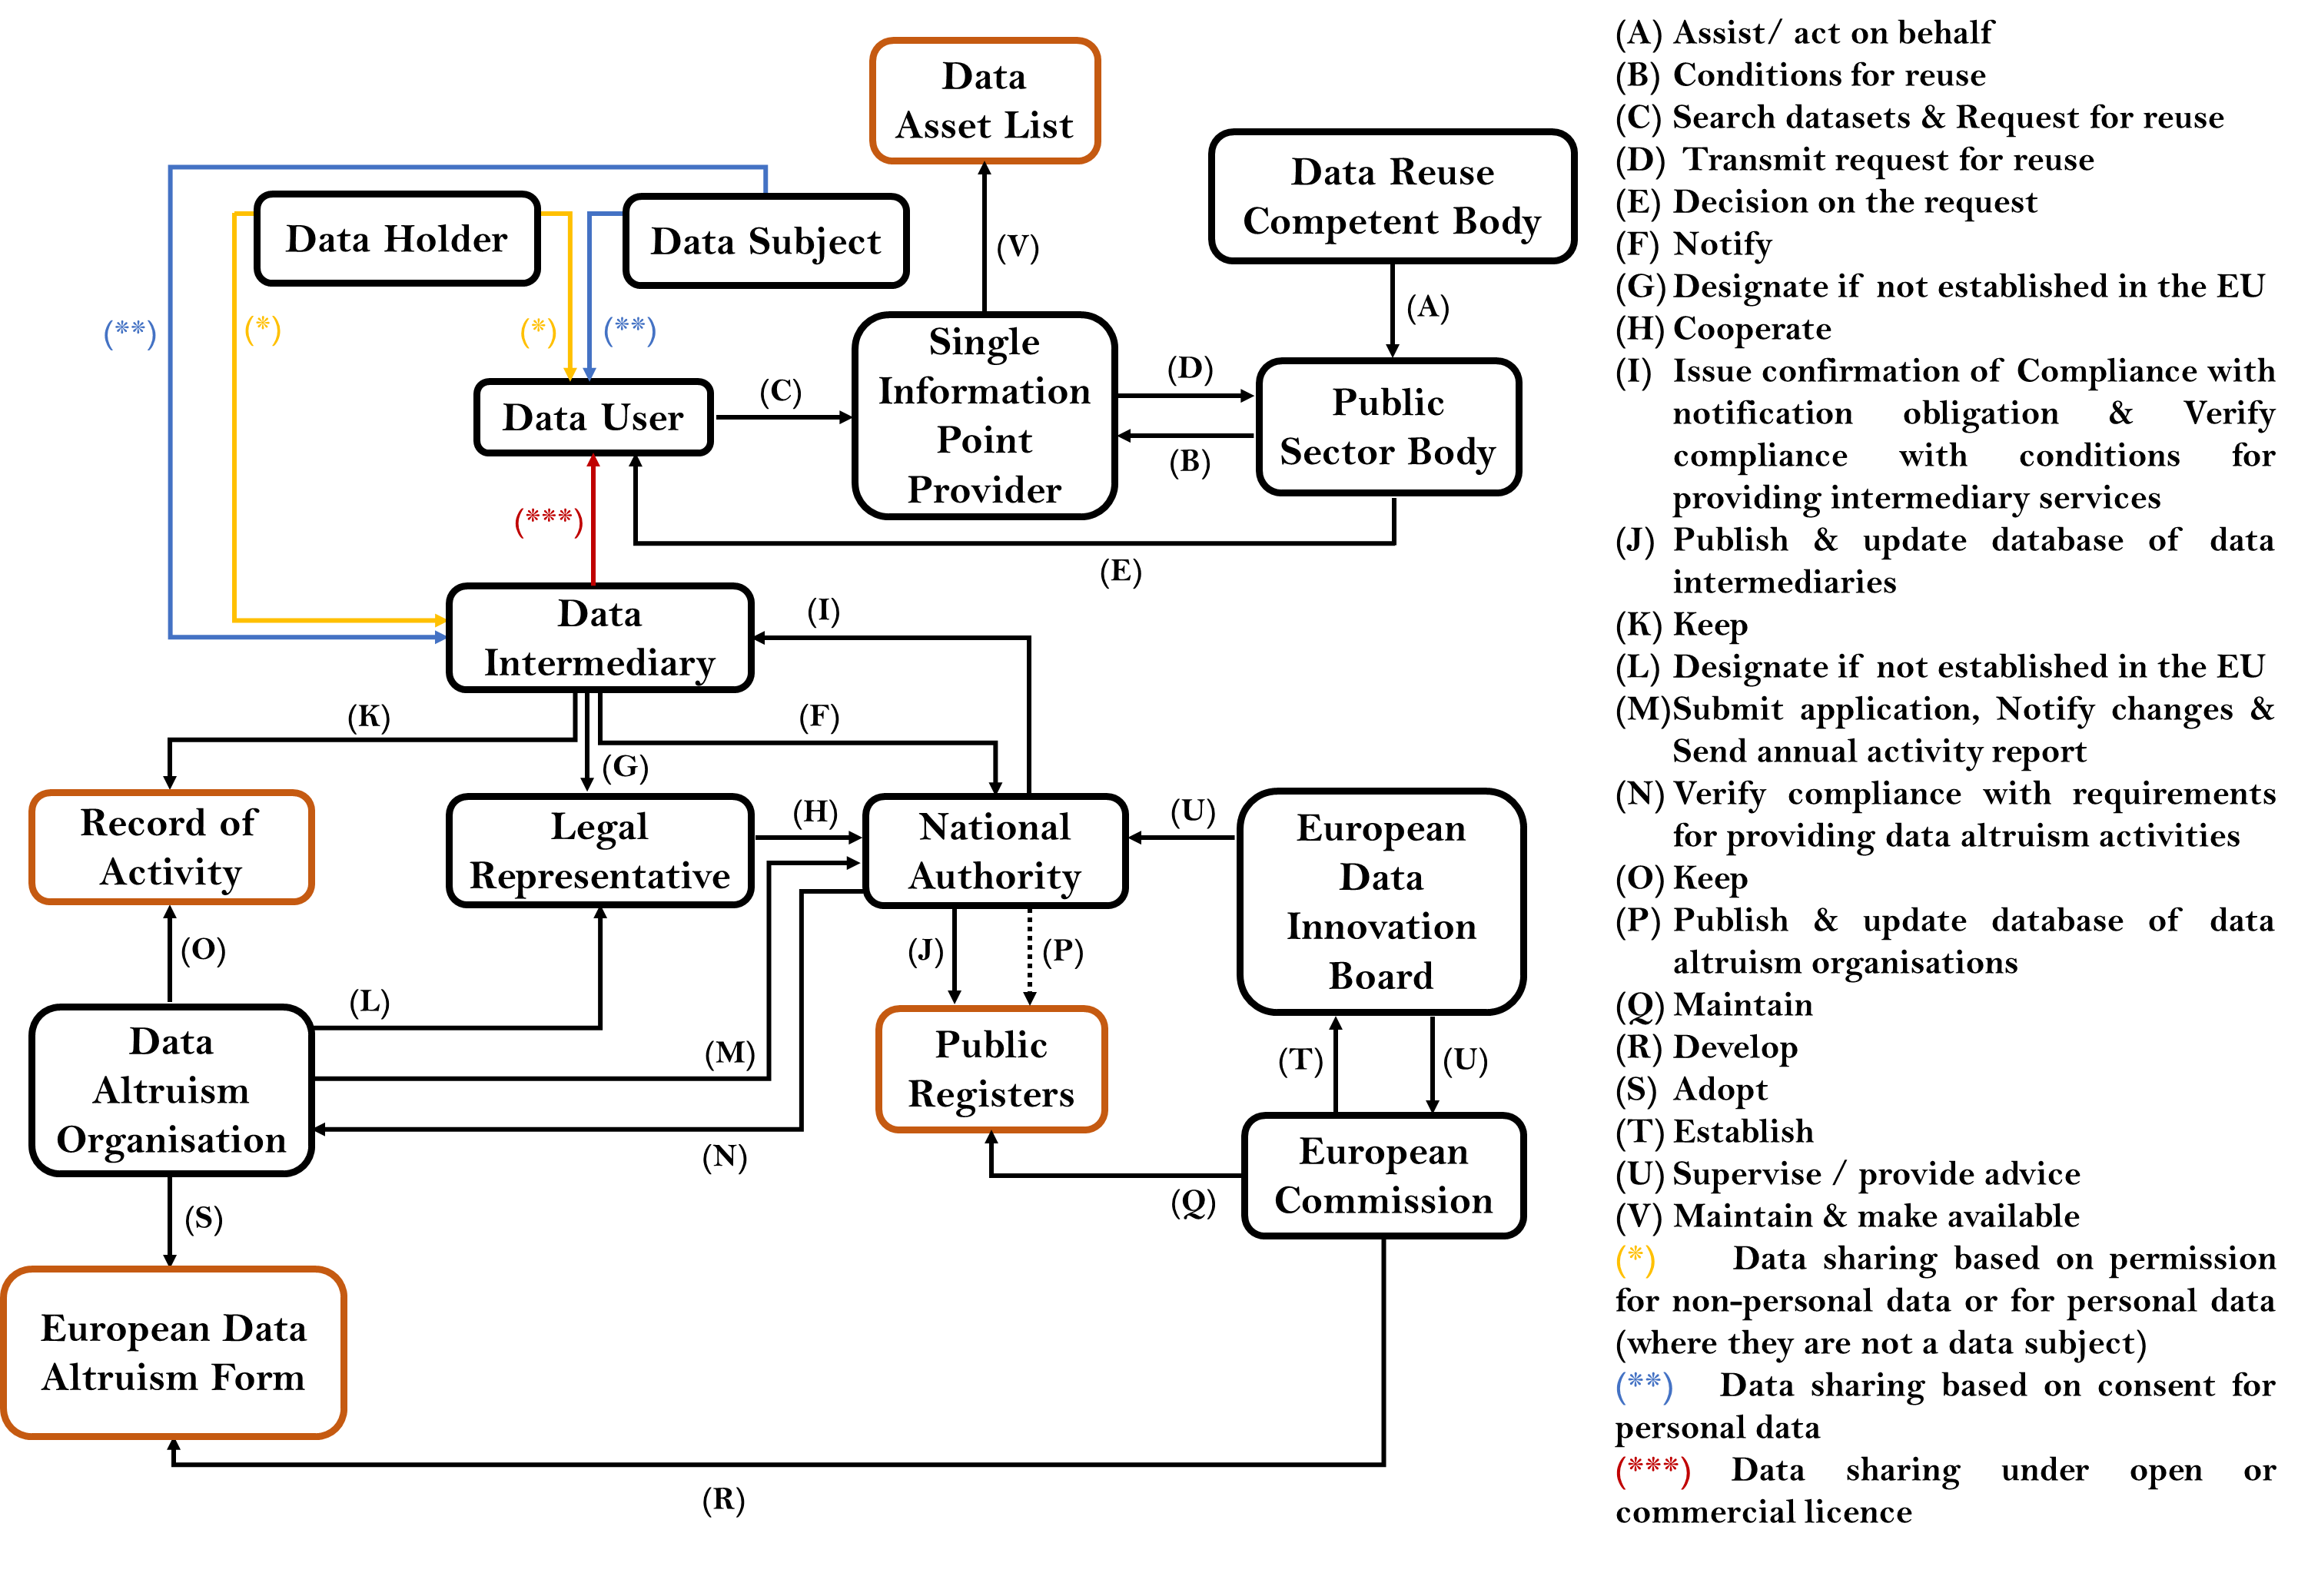
\includegraphics[width=\textwidth]{figures/chapter-7/information-flows.png}
\caption[Flows of information between DGA entities.]{Flows of information between DGA entities, adapted from \cite{esteves_semantics_2023}. The concepts in a black box are the (legal) entities and the ones in an orange box are the legal documentation that needs to be created and maintained by said entities. The direction of the arrows represents the direction of the information flow between entities. A short description of each flow is specified on the right side of the Figure.}
\label{fig:dga_flow}
\end{figure}

\subsection{Reuse of protected data held by public sector bodies}
\label{sec:reuse}

DGA's Chapter II legislates the reuse of data stored by public sector bodies.
To keep such data, these entities need to have in place safeguards to protect their commercial and statistical confidentiality, intellectual property rights of third parties, and personal data-related rights.
Moreover, they have to publish the dataset reuse conditions, and the respective data request procedure, in a transparent and publicly accessible manner.
The reuse must be contracted, with a maximum duration of one year, including the categories of data being used as well as the purpose for the reuse. 
Public sector bodies also have the right to obtain guidance and technical support from a competent body, which must be appointed by each EU member state.
These appointed entities are responsible for providing guidance on data formats and storage, assisting in the implementation of privacy-preserving methods to protect personal data integrity, and supporting activities to obtain consent from data subjects and permission from data holders.

\subsection{Data intermediaries}
\label{sec:intermediation}

DGA is also the first of its kind to regulate the activity of data intermediation service providers.
Such entities \textit{``aim[s] to establish commercial relationships for the purposes of data sharing between an undetermined number of data subjects and data holders on the one hand and data users on the other, through technical, legal or other means''} \citeyearpar{noauthor_regulation_2022}.
Article 12 includes a list of conditions for the provision of this service, e.g., providers should have tools to convert data into specific formats, use standards to promote interoperability across sectors, gather data subjects' consent and data holders' permission terms, as well as update or withdraw these terms, and maintain records of their activity.
Before providing this service, intermediation providers must be registered in the public register maintained by the EC, and their activity must be supervised at the national level by a nominated competent authority.

\subsection{Data altruism}
\label{sec:altruism}

Data altruism as a term is also introduced by the DGA.
This term relates to the sharing of personal and non-personal data, based on data subjects' consent and data holders' permission, for the `common good'.
This entails purposes such as improving healthcare, combating climate change, or performing scientific research.
Moreover, the proposed visions for an European Health Data Space \citeyearpar{noauthor_proposal_2022} and the Data Act \citeyearpar{noauthor_dataact_2022} also emphasise the altruistic reuse of data, with the Health Data Spaces proposal in particular focusing on the challenges brought on by the access and sharing of electronic health data for scientific research and public interest purposes.
In this context, each EU member state can establish its altruism policy and has to appoint a competent authority to oversee the activity of altruistic organisations (it can be the same as the one that supervises intermediation providers).
Said authority also has to keep up to date, public registries of altruistic organisations, including details on their identity, contact information, legal status, and main goals.
Data altruism organisations themselves have to maintain records of their activities, in particular, to produce annual reports to share with the relevant competent authority.
To facilitate this activity, a European data altruism consent form will be facilitated \beatriz{by the EC} to \textit{``allow the collection of consent or permission across Member States in a uniform format''} \citeyearpar{noauthor_regulation_2022}.

\subsection{European Data Innovation Board}
\label{sec:edib}

Aligned with the previously outlined regulatory objectives, the DGA established the formation of the European Data Innovation Board (EDIB), a supranational authority tasked with overseeing the operations of data intermediation service providers and data altruism organisations.
This Board comprises representatives from regulatory bodies overseeing data intermediation and altruism activities across all EU member states, from the EDPB and EDPS, from the European Union Agency for Cybersecurity (ENISA) and the European Commission, as well as experts in standardisation, portability, interoperability, and other pertinent stakeholders.
Article 30 \citeyearpar{noauthor_regulation_2022} delineates thirteen specific responsibilities of the EDIB, encompassing initiatives such as fostering uniform practices of data altruism throughout the EU and proposing guidelines for the development of common European data spaces.

% Figure of information flows and documents (from the paper)
% Comparison with GDPR flows
% Identification of important use cases that can be tackled and easily extended with the work already developed for GDPR